% This file was created by matlab2tikz.
%
%The latest updates can be retrieved from
%  http://www.mathworks.com/matlabcentral/fileexchange/22022-matlab2tikz-matlab2tikz
%where you can also make suggestions and rate matlab2tikz.
%
\definecolor{mycolor1}{rgb}{0.00000,0.44700,0.74100}%
\definecolor{mycolor2}{rgb}{0.85000,0.32500,0.09800}%
\definecolor{mycolor3}{rgb}{0.92900,0.69400,0.12500}%
\definecolor{mycolor4}{rgb}{0.49400,0.18400,0.55600}%
\definecolor{mycolor5}{rgb}{0.46600,0.67400,0.18800}%
%
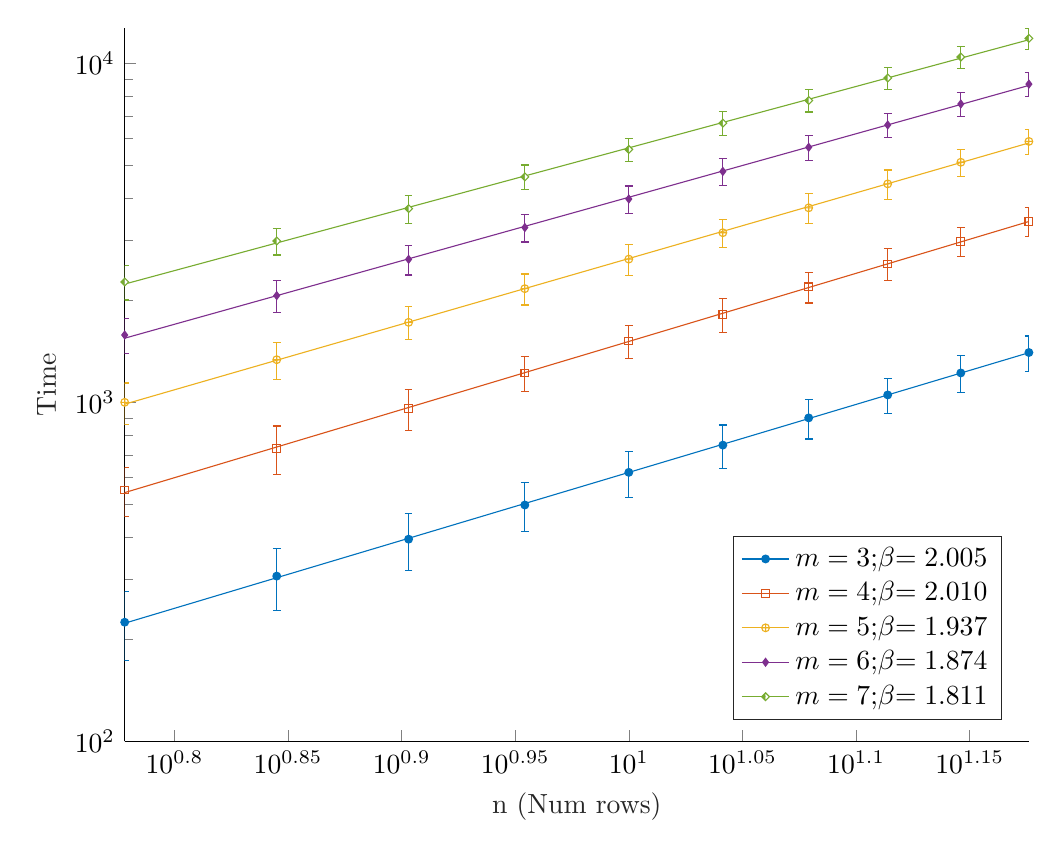
\begin{tikzpicture}

\begin{axis}[%
width=4.521in,
height=3.566in,
at={(0.758in,0.481in)},
scale only axis,
xmode=log,
xmin=6,
xmax=15,
xminorticks=true,
xlabel style={font=\color{white!15!black}},
xlabel={n (Num rows)},
ymode=log,
ymin=100,
ymax=12705.9256553665,
yminorticks=true,
ylabel style={font=\color{white!15!black}},
ylabel={Time},
axis background/.style={fill=white},
title style={font=\bfseries},
% title={$\text{Average ticks until solution as a function of n. On n }\times\text{ m grid. (k = 1)}$},
axis x line*=bottom,
axis y line*=left,
legend style={at={(0.97,0.03)}, anchor=south east, legend cell align=left, align=left, draw=white!15!black}
]
\addplot [color=mycolor1, draw=none, mark size=1.4pt, mark=*, mark options={solid, mycolor1}]
 plot [error bars/.cd, y dir = both, y explicit]
 table[row sep=crcr, y error plus index=2, y error minus index=3]{%
6	224.722	51.5852963702178	51.5852963702178\\
7	307.388	64.4326982300323	64.4326982300323\\
8	395.078	75.6178552728927	75.6178552728927\\
9	498.208	82.441360322253	82.441360322253\\
10	621.888	96.0689436804619	96.0689436804619\\
11	748.38	109.477496520924	109.477496520924\\
12	900.358	120.196790193189	120.196790193189\\
13	1052.224	125.687981770426	125.687981770426\\
14	1221.764	149.959862044645	149.959862044645\\
15	1403.72	166.445022427773	166.445022427773\\
};
\addlegendentry{$\text{m = 3; }\beta\text{ = 2.005}$}

\addplot [color=mycolor1, forget plot]
  table[row sep=crcr]{%
6	223.190492408606\\
7	304.042989387709\\
8	397.407164801274\\
9	503.292176185256\\
10	621.706101222408\\
11	752.656166691893\\
12	896.148911389444\\
13	1052.19030623361\\
14	1220.78584537807\\
15	1401.94061698218\\
};
\addplot [color=mycolor2, draw=none, mark size=1.4pt, mark=square, mark options={solid, mycolor2}]
 plot [error bars/.cd, y dir = both, y explicit]
 table[row sep=crcr, y error plus index=2, y error minus index=3]{%
6	551.422	90.6705808101443	90.6705808101443\\
7	731.714	120.193198701208	120.193198701208\\
8	958.91	133.170562428019	133.170562428019\\
9	1221.578	141.820951486588	141.820951486588\\
10	1517.23	168.773036281128	168.773036281128\\
11	1819.998	212.289867803303	212.289867803303\\
12	2192.036	226.506381777582	226.506381777582\\
13	2561.248	276.124196040982	276.124196040982\\
14	2982.672	292.432785926218	292.432785926218\\
15	3418.84	335.301285867814	335.301285867814\\
};
\addlegendentry{$\text{m = 4; }\beta\text{ = 2.010}$}

\addplot [color=mycolor2, forget plot]
  table[row sep=crcr]{%
6	541.975332284235\\
7	738.816033455425\\
8	966.261567791899\\
9	1224.35256794554\\
10	1513.12489535996\\
11	1832.61064984268\\
12	2182.83888834384\\
13	2563.83615508929\\
14	2975.62688390523\\
15	3418.23371083746\\
};
\addplot [color=mycolor3, draw=none, mark size=1.4pt, mark=oplus, mark options={solid, mycolor3}]
 plot [error bars/.cd, y dir = both, y explicit]
 table[row sep=crcr, y error plus index=2, y error minus index=3]{%
6	1000.742	140.324500236892	140.324500236892\\
7	1336.826	168.447394677232	168.447394677232\\
8	1723.12	193.333321355354	193.333321355354\\
9	2165.81	227.429431236119	227.429431236119\\
10	2647.382	272.465680720234	272.465680720234\\
11	3166.968	299.336170989283	299.336170989283\\
12	3750.928	375.702109344534	375.702109344534\\
13	4413.322	436.254308815305	436.254308815305\\
14	5111.72	458.259670329936	458.259670329936\\
15	5889.168	507.790533811391	507.790533811391\\
};
\addlegendentry{$\text{m = 5; }\beta\text{ = 1.937}$}

\addplot [color=mycolor3, forget plot]
  table[row sep=crcr]{%
6	988.236219845345\\
7	1332.05274802213\\
8	1725.19659202692\\
9	2167.25171656238\\
10	2657.85432505976\\
11	3196.68144432149\\
12	3783.44286557627\\
13	4417.87524530813\\
14	5099.73765873941\\
15	5828.80816618923\\
};
\addplot [color=mycolor4, draw=none, mark size=1.4pt, mark=diamond*, mark options={solid, mycolor4}]
 plot [error bars/.cd, y dir = both, y explicit]
 table[row sep=crcr, y error plus index=2, y error minus index=3]{%
6	1580.908	188.985986099191	188.985986099191\\
7	2065.948	221.5611337034	221.5611337034\\
8	2643.466	266.092651989652	266.092651989652\\
9	3280.572	306.39017395045	306.39017395045\\
10	3984.212	366.009646291401	366.009646291401\\
11	4803.128	429.887988878456	429.887988878456\\
12	5658.464	470.425859922014	470.425859922014\\
13	6586.044	543.183673420087	543.183673420087\\
14	7594.482	637.759028813915	637.759028813915\\
15	8690.702	701.464483805189	701.464483805189\\
};
\addlegendentry{$\text{m = 6; }\beta\text{ = 1.874}$}

\addplot [color=mycolor4, forget plot]
  table[row sep=crcr]{%
6	1547.20017105432\\
7	2065.35142144417\\
8	2652.53720795416\\
9	3307.60040337575\\
10	4029.53721333458\\
11	4817.46276256627\\
12	5670.58697584018\\
13	6588.1970370611\\
14	7569.6442451874\\
15	8614.33391851345\\
};
\addplot [color=mycolor5, draw=none, mark size=1.4pt, mark=halfsquare left*, mark options={solid, mycolor5}]
 plot [error bars/.cd, y dir = both, y explicit]
 table[row sep=crcr, y error plus index=2, y error minus index=3]{%
6	2266.826	260.977727925097	260.977727925097\\
7	2994.622	271.02790884103	271.02790884103\\
8	3730.682	352.494586828631	352.494586828631\\
9	4628.37	388.318476999432	388.318476999432\\
10	5576.252	435.161809096562	435.161809096562\\
11	6667.926	539.045174288619	539.045174288619\\
12	7777.73	584.595090588246	584.595090588246\\
13	9060.382	684.749241052697	684.749241052697\\
14	10444.846	762.089855712803	762.089855712803\\
15	11855.372	850.5536553665	850.5536553665\\
};
\addlegendentry{$\text{m = 7; }\beta\text{ = 1.811}$}

\addplot [color=mycolor5, forget plot]
  table[row sep=crcr]{%
6	2234.71419827863\\
7	2954.42646859737\\
8	3762.75334040737\\
9	4657.48041858003\\
10	5636.70195196142\\
11	6698.74975621778\\
12	7842.14375887224\\
13	9065.5562646807\\
14	10367.7853345205\\
15	11747.7344471407\\
};
\end{axis}
\end{tikzpicture}%
